\newchapter{Hardware}
\newsection{Processor VS CPU VS Core}
\index{Processor}
\index{CPU}
\index{Core}
\label{processorcpucore}
\begin{itemize}
    \item \textbf{Processor} is a~general name of~any gadget that can read instructions and~perform actions according to~these instructions (i.e.,~that can process instructions).
    \item \textbf{CPU} (Central Processing Unit) is a~specific type of~processor. It's the main processor in a~computer controlling the~behavior of~all other parts of the~computer. Nowadays CPU is treated as a~synonym of the~processor, but that's wrong. Beside the~CPU there are~other processors in a~computer. For~example, a~hard drive contains its own processor controlling data reading and~writing, graphic cards contain a~GPU (Graphics Processing Unit) performing calculations needed to render and~display images etc.
    \item \textbf{Core} is the main computation component of the CPU performing instructions (with the~help of~other parts of the~core like \hyperref[alu]{ALUs}). Typically, one core can process one instruction at~a~time, although nowadays there are even cores enabling parallel instructions processing. However, usually the~parallelism is still achieved by putting more cores to one CPU and~more CPUs to~one computer. For~example, when you read the~typical "state--of--the--art" claim that a~computer has~quad--core processor, it means that there is a~single CPU with four cores in the~computer. Beside cores CPUs also contain switch bridges (distributing instructions to~cores), caches and~other stuff.
\end{itemize}

\newsection{ALU}
\index{ALU}
\index{Arithmetic logic unit}
\index{Logic gate}
\label{alu}
The~abbreviation stands for~\textit{Arithmetic Logic Unit}. It's an electronic circuit that performs arithmetic and~bitwise operations on~integer binary numbers.

\warning Do not confuse it with a~simple electronic device performing a~boolean operation over two bits (AND, OR, XOR etc.). That's called \textit{Logic Gate}. An~ALU consists of multiple logic gates.

\warning ALUs are parts of~CPUs, but not cores. A~core is connected with an~ALU via an~execution port, sends inputs to it and processes returned results.

\begin{figure}
    \centering
    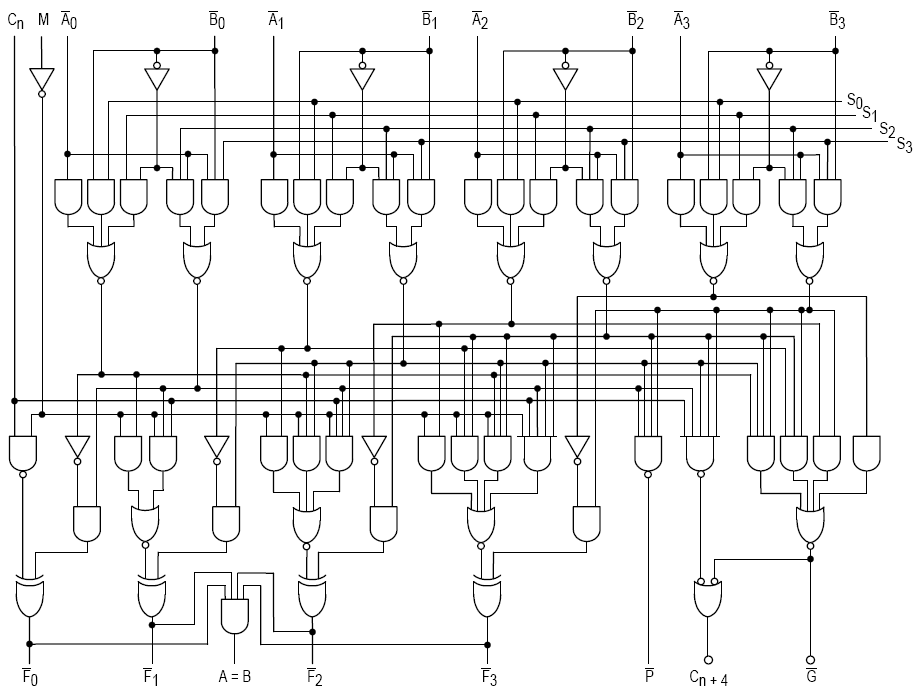
\includegraphics[width=\textwidth]{ALU.png}
    \caption*{An example of a simple (no joke) four--bit ALU}
\end{figure}
\newpage

\newsection{System Memory}
\index{System memory}
\index{Computer memory}
\index{Memory}
\label{systemmemory}
System memory, also computer memory or~maliciously simply memory, is a~memory from which a~\hyperref[processorcpucore]{processor} reads a~\hyperref[applicationprocessprogramservicethread]{process} instructions and~other data that the~process requires. I.e.,~to~run a~process the~computer \hyperref[os]{OS} must load its instructions and~required data to~the~system memory, from which the~computer processor can~read~them and~subsequently process~them.

System memories are~almost every time \hyperref[ram]{RAMs} because of~the~fast access to~any of~stored data. That's why you can often meet the~"state--of--the--art" claim that a~computer has~16~GB of~RAM, but~that isn't accurate. It~means that the~computer memory can hold up~to~16~GB of~data at~a~time and~the~memory is the~\hyperref[ram]{RAM} type.

\warning Memory doesn't mean \hyperref[harddiskdrive]{hard disk} (permanent computer memory). That's called \hyperref[harddiskdrive]{\textit{storage}}.

\newsection{32b VS 64b}
\index{32b}
\index{64b}
\index{General purpose registry}
\index{GPR}
\label{32bvs64b}
The~number denotes the~bit size of~the~general purpose registry of~a~computer processor. You~can~encounter a~claim that there~is 32b or~64b processor. \textit{General purpose registry (GPR)}~is a~small, very fast memory that the~processor uses for~addressing locations in~the~\hyperref[systemmemory]{system memory}. Consider the~content of~the~GPR as~one~value. Each~single value stored in~the~GPR identifies one~bit of~the~\hyperref[systemmemory]{system memory}.

A~32b~GPR can store only $2^{32}$ values, which means it's~capable~of addressing only exactly 4\,GB (when~$1\,\textrm{GB}=2^{30}\,\textrm{B}$) of~the~\hyperref[systemmemory]{system memory}. I.e.,~with a~32b~processor it~doesn't matter how big \hyperref[systemmemory]{system memory} you~have, you~can~use maximally~4\,GB. And~that sucks with today's available~\hyperref[ram]{RAMs}.

But~a~64b~GPR can store $2^{64}$ values, which means it's~theoretically capable~of addressing approximately 18~billion~GB of~the~\hyperref[systemmemory]{system memory}. And~that's more than enough to~fully leverage even the~largest available~\hyperref[ram]{RAMs}.

\newsection{Hard Disk VS Hard Drive}
\index{Hard disk}
\index{Hard drive}
\index{Hard disk drive}
\index{HDD}
\label{harddiskdrive}
There's no~difference between these two terms. They both denote a~permanent data storage of~a~computer. To~make things even more complicated, even the~composed term \textit{hard disk drive} is~used for~it. And~that's where the~abbreviation \textit{HDD} comes from.

\newsection{Random Access Memory (RAM)}
\index{Random Access Memory}
\index{RAM}
\label{ram}
It's~a~type of~volatile data storage consisting~of computer chips. Its~main advantage is a~very short access time to~any~stored data (much~faster in~comparison to~\hyperref[harddiskdrive]{hard disks}). On~the~other side, its~disadvantages are~the~volatility (when the~computer is~turned~off, all~data are~lost) and~small capacity. RAM~memories are~usually used as~\hyperref[systemmemory]{system memories}.
